\documentclass[tikz,convert={density=300,outext=.png}]{standalone}
\usetikzlibrary{arrows.meta,graphs}
\usepackage{amsmath}
\begin{document}
    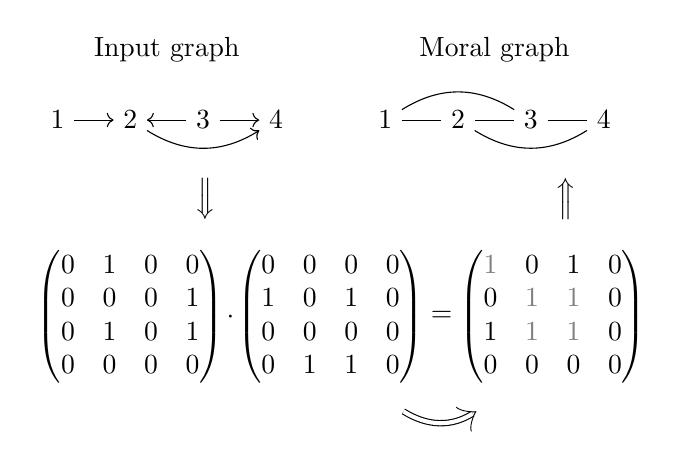
\begin{tikzpicture}[xscale=0.925]
      \node (lg) at (1.5,0.9) {Input graph};
      \node (lm) at (6,0.9) {Moral graph};

      \node (1) at (0,0) {$1$};
      \node (2) at (1,0) {$2$};
      \node (3) at (2,0) {$3$};
      \node (4) at (3,0) {$4$};

      \graph[use existing nodes] {
        1 -> 2;
        3 -> 2;
        2 ->[bend right] 4;
        3 -> 4;
      };

      \node (1) at (4.5,0) {$1$};
      \node (2) at (5.5,0) {$2$};
      \node (3) at (6.5,0) {$3$};
      \node (4) at (7.5,0) {$4$};

      \graph[use existing nodes] {
        1 -- 2;
        1 --[bend left] (3);
        3 -- 2;
        2 --[bend right] 4;
        3 -- 4;
      };

      \node (A) at (1,-2.5) {$\begin{pmatrix} 0 & 1 & 0 & 0 \\ 0 & 0
          & 0 & 1 \\ 0 & 1 & 0 & 1 \\ 0 & 0 & 0 & 0  \end{pmatrix}$};
      \node (B) at (3.75,-2.5) {$\begin{pmatrix} 0 & 0 & 0 & 0 \\ 1 & 0
          & 1 & 0 \\ 0 & 0 & 0 & 0 \\ 0 & 1 & 1 & 0  \end{pmatrix}$};
            \node (C) at (6.8,-2.5) {$\begin{pmatrix} \color{gray}{1}
            & 0 & 1 & 0 \\ 0 & \color{gray}{1}
            & \color{gray}{1} & 0 \\ 1 & \color{gray}{1} &
              \color{gray}{1} & 0 \\ 0 & 0 & 0 & 0  \end{pmatrix}$};

          \node (cdot) at (2.375, -2.5) {$\cdot$};
        \node (eq) at (5.275, -2.5) {$=$};

      \draw[double distance =1.5pt, -{Classical TikZ Rightarrow}]
      (4.75, -3.7) to[bend right] (5.75, -3.7);
      \node[rotate=270] at (2,-1) {$\Longrightarrow$};
      \node[rotate=90] at (7,-1) {$\Longrightarrow$};
  \end{tikzpicture}
\end{document}


